% !TeX root = ./9-handout.tex

%\item<2-> % reveals second and keeps on page in subsequent frames
%\begin{itemize}[<2->] %does for a whole list of items

%joke I have to make haha: we could spend a whole semester on incompleteness/computability, so obviously our treatment will be incomplete (and the theorem tells us we can't do better!). funny to think that one can in a sense give a complete treatment of incompleteness. 

%topic 9: constructive math
%connection w/ computable math
%could prove undecidability of predicate logic? e.g. gordon notes? 
%lots of b-days: komolgorov, wittgenstein, godel 
%do mental health resources? 
%be chill: can cover essentials in two days tops and still a day's worth of slides on probability. so be chill. at this point, those who were responsible don't need to come to class anymore. so people are opting in. 

%could do reductio proofs! 
%changes to notion of rigor in mathematics; e.g. bolzano moving away from physical intuition , motion, passage of time. 


%topic 10: hilbert's program formalism
%glitch interpretation of axiom of choice 

%could also do intuitionism; how this fits in


% % One philosophically interesting point that I probably should have emphasized while introducing Turing machines: it is fascinating that in some sense these are the basic or fundamental constituents of any computation. E.g., it is hard to imagine how we could break down computation into smaller components than that given by a Turing machine.
% This could be an interesting philosophy prompt question: can you think of breaking a computation into smaller pieces than those given by a Turing machine?
% Presumably there are other ways to decompose computation that presumably end up being equivalent to computation by Turing machines.

% E.g. very interesting quotation from Turing 1936 paper, quoted by Smith pages 342-343: Turing says ``imagine the operations performed by the [human] computer to be split up into `simple operations' which are so elementary that it is not easy to imagine them further divided" [quoted by Smith on page 342]
% a lot of the quotations from section 9 of this paper are fascinating. Really does a good job motivating the simplicity of Turing machines.


%Notes on non-determinisitic Turing machines: seems that we can always simulate these with a deterministic TM, although the computational complexity can be different:
%``Any  computational  problem  that  can  be  solved  by  a  DTM  can  also  be  solved  by  a NTM, and vice versa. However, it is believed that in general the time complexity may not be the same."
% The P = NP problem, the most famous unresolved question in computer science, concerns one case of this issue: whether or not every problem solvable by a NTM in polynomial time is necessarily also solvable by a DTM in polynomial time."
%https://en.wikipedia.org/wiki/Nondeterministic_Turing_machine

%on relation to quantum computers:
%``it is believed by experts (but has not been proven) that the power of quantum computers is, in fact, incomparable to that of NTMs; that is, problems likely exist that an NTM could efficiently solve that a quantum computer cannot and vice versa"
%``In particular, it is likely that NP-complete problems are solvable by NTMs but not by quantum computers in polynomial time"


\setcounter{section}{8} 

\section{Computability Theory}
%\subsection*{test}

\begin{frame}
%\large

\scriptsize{\tableofcontents}

\end{frame}

%\iffalse %********************************************************************************


\begin{frame}
\frametitle{Liable to forget:}
%\large

\begin{itemize}[<+->]


\item No Pset due this Sunday April 30th!

\item PSet 9 is due next Sunday May 7th, 5pm!

\item Only one PSet left after this (due May 14th). Which you can drop if you've turned in all prior psets! 

\item Feel free to join \href{https://piazza.com/mit/spring2023/24118}{Piazza}! 

\item Feel free to join PSet partners!
\item[] Groups will be auto-assigned Thursday 


\end{itemize}
\end{frame}

\subsection{Motivation}

\begin{frame}
\frametitle{Non-computable Functions}
%\large

\begin{itemize}[<+->]

\item We'll focus on functions $f: \mathbb{N} \rightarrow \mathbb{N}$.

\item For a computer program to \emph{compute} $f$ is for it to yield $f(n)$ as output whenever it is given $n$ as input ($n \in \mathbb{N}$). 

\item \emph{Theorem:} not every function is computable (e.g. Halting function).

%we'll use this idea to prove Godel's theorem in next topic!

\end{itemize}
\end{frame}

\begin{frame}
\frametitle{Plan of Attack}
%\large

\begin{itemize}[<+->]

\item Turing Machines are computers of an especially simple sort.

\item We'll see that some functions are not Turing-computable.

\item But: any function that can be computed using an ordinary computer is also computed by some Turing Machine 
%by one direction of the `fundamental theorem of Turing machines'

\item So some functions are not computable 

\end{itemize}
\end{frame}

\begin{frame}
\frametitle{Fundamental Theorem of Turing Machines}
%\large

One reason Turing Machines are so valuable:

\begin{itemize}[<+->]

\item \emph{Fundamental Theorem of Turing Machines}: A function from natural numbers to natural numbers is Turing-computable if and only if it can be computed by an ordinary computer, assuming unlimited memory and running time.

\item  One shows that every Turing-computable function is computable by an ordinary computer (given unlimited memory and running time) by showing that one can program an ordinary computer to simulate any given Turing Machine.

\item  One shows that every function computable by an ordinary computer (given unlimited memory and running time) is Turing-computable by showing that one can find a Turing Machine that simulates any given ordinary computer.

% potentially interesting philosophical question: what does it mean to simulate one thing by another? Is this a special kind of representation relation?

\end{itemize}
\end{frame}

\begin{frame}
  \frametitle{Happy Birthday to Kolmogorov!}

  \begin{columns}
    \begin{column}{.35\textwidth}
      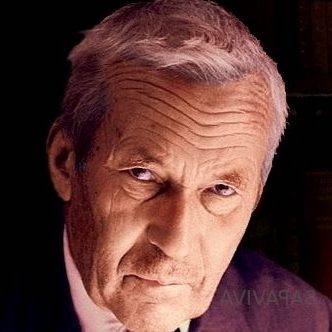
\includegraphics[height=.6\textheight]{../assets/Kolmogorov}
    \end{column}
    \begin{column}{.7\textwidth}
      \begin{itemize}[<+->]
        \item Andrey Kolmogorov (1903--1987)
                
        \item Soviet mathematician: axiomatized probability theory (early 1930s) 
        
        \item 1920s: Fourier series and intuitionistic logic (pre Ph.D.)
        
        \item 1940s: stochastic processes and war stuff\dots
        %turbulence 
        
        \item 1950s: classical mechanics! 
        %dynamical systems. KAM theorem
        
        \item 1960s: information theory, Kolmogorov complexity!
        %``In algorithmic information theory (a subfield of computer science and mathematics), the Kolmogorov complexity of an object, such as a piece of text, is the length of a shortest computer program (in a predetermined programming language) that produces the object as output. It is a measure of the computational resources needed to specify the object, and is also known as algorithmic complexity, Solomonoff–Kolmogorov–Chaitin complexity, program-size complexity, descriptive complexity, or algorithmic entropy. It is named after Andrey Kolmogorov, who first published on the subject in 1963[1][2] and is a generalization of classical information theory.''
     
      \end{itemize}
    \end{column}
  \end{columns}
\end{frame}

\begin{frame}
  \frametitle{Happy Birthday to Wittgenstein tm!}

  \begin{columns}
    \begin{column}{.35\textwidth}
      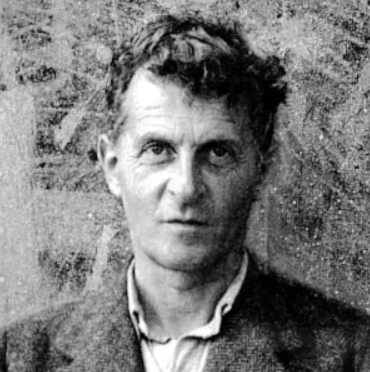
\includegraphics[height=.6\textheight]{../assets/Wittgenstein}
    \end{column}
    \begin{column}{.7\textwidth}
      \begin{itemize}[<+->]
        \item Ludwig Wittgenstein (1889--1951)
                
        \item Austrian philosopher (most influential of 20th century!) 
        
        \item WWI: \textit{Tractatus Logico-Philosophicus}
        
        \item 1930s: \textit{Blue and Brown Books}
        
        \item 1950s: \textit{Philosophical Investigations} and \textit{Remarks on Foundations of Mathematics}
        
      %  \item Rule-following paradox: relevant for interpreting Turing Machines, e.g. Church--Turing thesis. e.g. is anything an effective method or algorithmic? e.g. not requiring any creativity?
     
      \end{itemize}
    \end{column}
  \end{columns}
\end{frame}

\subsection{Turing Machines}

\begin{frame}
\frametitle{Hardware: the cheap part}
%\large

\begin{itemize}[<+->]

\item \emph{Memory tape}: A long strip of paper, divided into cells:

\bigskip

\begin{center}
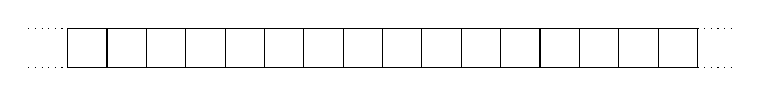
\begin{tikzpicture}
\draw (0,0) -- (8,0); % base horizontal
\draw[dotted] (8,0) -- (8.5,0); % base horizontal dots (right)
\draw[dotted] (-0.5,0) -- (0,0); % base horizontal dots (left)
\draw (0,0.5) -- (8,0.5); % top horizontal
\draw[dotted] (8,0.5) -- (8.5,0.5); % top horizontal dots (right)
\draw[dotted] (-0.5,0.5) -- (0,0.5); % top horizontal dots (left)


\draw (0,0) -- (0,0.5); % vertical
\draw (0.5,0) -- (0.5,0.5); % vertical
\draw (1,0) -- (1,0.5); % vertical
\draw (1.5,0) -- (1.5,0.5); % vertical
\draw (2,0) -- (2,0.5); % vertical
\draw (2.5,0) -- (2.5,0.5); % vertical
\draw (3,0) -- (3,0.5); % vertical
\draw (3.5,0) -- (3.5,0.5); % vertical
\draw (4,0) -- (4,0.5); % vertical
\draw (4.5,0) -- (4.5,0.5); % vertical
\draw (5,0) -- (5,0.5); % vertical
\draw (5.5,0) -- (5.5,0.5); % vertical
\draw (6,0) -- (6,0.5); % vertical
\draw (6.5,0) -- (6.5,0.5); % vertical
\draw (7,0) -- (7,0.5); % vertical
\draw (7.5,0) -- (7.5,0.5); % vertical
\draw (8,0) -- (8,0.5); % vertical


\end{tikzpicture}
\end{center}

\bigskip

\item A unionized assistant stands ready to add paper on either end

\end{itemize}
\end{frame}

\begin{frame}
\frametitle{Hardware: the fancy part}
%\large

\begin{itemize}[<+->]

\item \emph{Tape-reader}: at each step, a reader is positioned on a cell of the memory tape and is able to perform any of the following functions: 

      \begin{itemize}
      \item Read the symbol written on the cell (e.g. a blank, `0', or `1')
      \item Erase or write a new symbol on the cell 
      \item Move one cell to the left ($\ell$)
      \item Move one cell to the right ($r$)
      \end{itemize}

\item \textbf{Hardware Setup}: a set $Q = \{ q_0, q_1, \dots, q_f \}$ ($f \geq 0$) of states, with an initial state $q_0 = 0$ and a halting state $q_f$. 

\end{itemize}

\end{frame}

\begin{frame}
\frametitle{Software (list of if-then statements)}
%\large

\begin{itemize}[<+->]

\item A finite list of \textbf{command lines} $c_k$:
\[
\seq{\text{current state}} \seq{\text{current symbol}} \seq{\text{new symbol}} \seq{\text{direction}} \seq{\text{new state}}
\]
\item Think of a command line as encoding the following instruction:

\item[] If you are in $\seq{\text{current state}}$ and the reader sees $\seq{\text{current symbol}}$ written on the memory tape, replace $\seq{\text{current symbol}}$ with $\seq{\text{new symbol}}$. 
\item[] -- Then move one step in $\seq{\text{direction}}$, and go to $\seq{\text{new state}}$.

\item \textit{Mnemonic}: convention tracks time-order of steps left to right

\end{itemize}
\end{frame}

\begin{frame}
\frametitle{Formal-ware}
%\large

\begin{itemize}[<+->]

\item \emph{Software}: a set of commands for a given hardware setup such that no two commands are inconsistent

\item \emphz{Inconsistent commands}: two commands $c_1 = \langle q_{1i}, s_{1i}, s_{1f}, d_1, q_{1f}\rangle$ and $c_2 = \langle q_{2i}, s_{2i}, s_{2f}, d_2, q_{2f}\rangle$ are \textbf{inconsistent} provided $\textcolor{highlightA}{q_{1i}} = \textcolor{highlightA}{q_{2i}}$ and $\textcolor{highlightB}{s_{1i}} = \textcolor{highlightB}{s_{2i}}$ but $c_1 \neq c_2$

\item[] e.g. $c_1 = \langle \textcolor{highlightA}{3}, \textcolor{highlightB}{1}, 0, r, 4\rangle$ and $c_2 = \langle \textcolor{highlightA}{3}, \textcolor{highlightB}{1}, $ \emphz{1}$, r, 4\rangle$

\item \textbf{Turing Machine}: a hardware setup together with software for it 

\end{itemize}


\end{frame}

\begin{frame}
\frametitle{Operating a Turing Machine (a.k.a. Drill baby Drill)}
%\large

\begin{itemize}[<+->]

\item \textbf{Operation}: begin in State 0 (or whatever is the initial state $q_0$)

\item Then carry out the following procedure, for as long as you can:
%better: for as many steps as possible. 

\item Perform the instruction corresponding to the (first) command line that matches your current state and the symbol on which your reader is positioned

\item (Rinse \&) Repeat

\item If you cannot go on, Halt. 
%\item If you are unable carry out the procedure, halt.
%what does it mean to not be able to go on!? to not be able to carry out a rule any longer. 

\end{itemize}
\end{frame}

\begin{frame}
\frametitle{A Turing Machine Simulator}
%\large

\begin{itemize}[<+->]

\item \href{http://morphett.info/turing/}{morphett}

\item Follows our conventions for command lines, with a few bells and whistles 

\end{itemize}
\end{frame}

\begin{frame}
\frametitle{Philosophy Prompt \#19: Merely convenient?}
%\large

\begin{itemize}[<+->]

\item Nobody codes anything practical using Turing machines, but standard computer languages do not add expressive power over Turing Machines

\item[] -- e.g. anything we can compute using $C^{++}$, Python, JavaScript, etc. can be programmed using a Turing Machine

\item \emph{Question}: are more sophisticated programming languages \textit{merely convenient}, or do they add something more valuable than efficiency, ease-of-use, or some other practical consideration?

\item[] -- If so, what kind of value does this `something more' have?


\end{itemize}
\end{frame}

\subsection{Turing Numbers}

\begin{frame}
\frametitle{Turing Computabiity}
%\large

\begin{itemize}[<+->]

\item $M$ \emph{computes} a function \(f(x)\) if and only if it delivers \(f(n)\) as output whenever it is given $n$ as input.


\item $M$ takes \(n\) ($n \in \mathbb{N}$) as \textbf{input} if it starts out with a tape that contains only a sequence of \(n\) ones (with the reader positioned at the left-most one, if $n > 0$).

\item  $M$ delivers \(f(n)\) as \textbf{output} if it halts with a tape that contains only a sequence of \(f(n)\) ones (with the reader positioned at the left-most one, if $n > 0$).


\end{itemize}
\end{frame}

\begin{frame}
  \frametitle{Happy Birthday to G{\"o}del tomorrow!}

  \begin{columns}
    \begin{column}{.35\textwidth}
      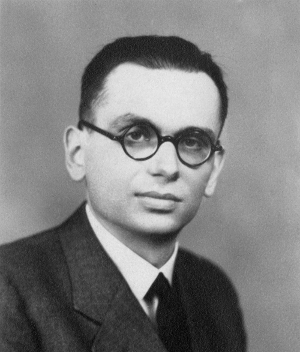
\includegraphics[height=.6\textheight]{../assets/goedel}
    \end{column}
    \begin{column}{.7\textwidth}
      \begin{itemize}[<+->]
        \item Kurt G{\"o}del (1906--1978)
                
        \item[] 'nuff said!

%fascinating how Godel initially intended to study physics but interactions w/ philosophers (e.g. vienna circle) and a class by Moritz Schlick covering Russell's ``intro to math philosophy" led Godel to change gears to study mathematical logic! so that's one good thing philosophy has done haha. 
%``According to Gödel, mathematical logic was "a science prior to all others, which contains the ideas and principles underlying all sciences." " 
        
        \item[1929:] Completeness of First order Logic
        
        \item[1931:] Incompleteness of Arithmetic    

\item[1938:] Consistency of Axiom of Choice with ZF, and of Continuum Hypothesis with ZFC  

\item[1949:] closed timelike curves!   
     
      \end{itemize}
    \end{column}
  \end{columns}
\end{frame}

\begin{frame}
  \frametitle{Happy Birthday to Gauss on Sunday!}

  \begin{columns}
    \begin{column}{.35\textwidth}
      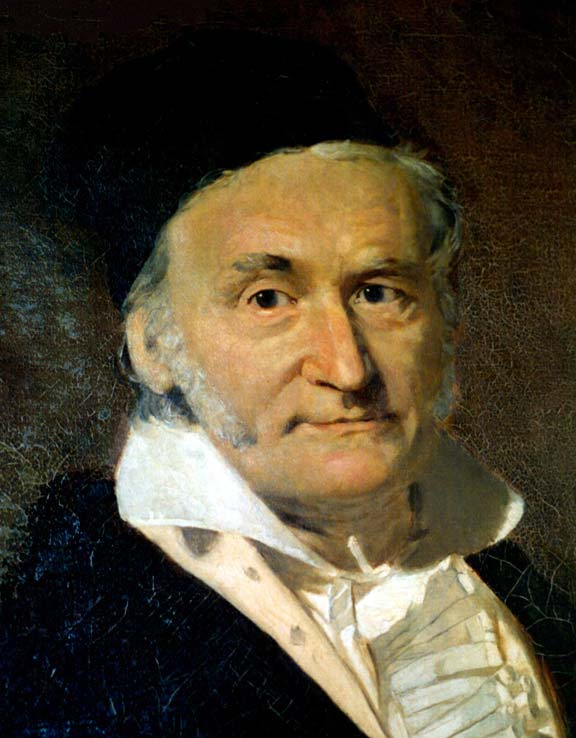
\includegraphics[height=.6\textheight]{../assets/gauss}
    \end{column}
    \begin{column}{.7\textwidth}
      \begin{itemize}[<+->]
        \item Carl Friedrich Gauss (1777--1855)
                
        \item the greatest of all time?
        
           \item Number theory, algebra    

     \item Astronomy 
        
        \item Non-euclidean Geometry
%https://www.cut-the-knot.org/triangle/pythpar/Drama.shtml
        
        \item 1805: Fast Fourier Transform
% surely part of this claim must be anachronistic!
% Great example for computability theory unit: FFT is basically an algorithmic speed up of computing the discrete Fourier transform (DFT)
% whereas the computational complexity of computing the DFT is O(N^2). The computational complexity of the Fast Fourier Transform is O(N log N), where N is the data size. 
%``The FFT's importance derives from the fact that it has made working in the frequency domain equally computationally feasible as working in the temporal or spatial domain"

%epistemic component (minimizing error): ``In the presence of round-off error, many FFT algorithms are much more accurate than evaluating the DFT definition directly or indirectly"

%``The development of fast algorithms for DFT can be traced to Carl Friedrich Gauss's unpublished work in 1805 when he needed it to interpolate the orbit of asteroids Pallas and Juno from sample observations.[6][7] His method was very similar to the one published in 1965 by James Cooley and John Tukey, who are generally credited for the invention of the modern generic FFT algorithm"

%``1994, Gilbert Strang described the FFT as "the most important numerical algorithm of our lifetime",[3][4] and it was included in Top 10 Algorithms of 20th Century by the IEEE magazine Computing in Science & Engineering."
        
   
        
         
     
      \end{itemize}
    \end{column}
  \end{columns}
\end{frame}

\begin{frame}
\frametitle{Coding Turing Machines as Numbers}
%\large

\begin{itemize}[<+->]

\item To prove various results, we code each non-empty Turing Machine as a unique natural number
%we code the empty turing machine as a bunch of natural numbers, all those not arising from our coding procedure. 

\item We can then run one Turing Machine as input through another TM

\item For simplicity, we'll focus on \textbf{one symbol} Turing Machines: \\ only admissible symbols are ones and blanks

\item[] And we'll assume that the tape is only unbounded on the right
% not sure where this assumption figures in the proofs

\item[] In the PSet, you are not restricted in these ways! 

\item \textbf{Plan}: $\text{Turing Machine} \rightarrow \text{Sequence of symbols} \rightarrow
\text{Sequence of numbers} \rightarrow  \text{Unique number}$


\end{itemize}
\end{frame}

\begin{frame}
\frametitle{$\text{Sequence of symbols} \rightarrow \text{Sequence of numbers}$}
%\large

\begin{multicols}{3}

\begin{center}State Symbols:
\end{center}
\[
\begin{array}{ccc}
\text{``0''} &\rightarrow &\text{0}\\
\text{``1''} &\rightarrow &\text{1}\\
 &\vdots &
\end{array}
\]

\pause

\columnbreak

\begin{center}Tape Symbols:
\end{center}
\[
\begin{array}{ccc}
\text{``\ub''} &\rightarrow &\text{0}\\
\text{``$1$''} &\rightarrow &\text{1}\\
\
\end{array}
\]

\columnbreak

\pause
\begin{center}Movement Symbols: \vspace{-2em}
\end{center}
\[
\begin{array}{ccc}
\text{``r''} &\rightarrow &\text{0}\\
\text{``$*$''} &\rightarrow &\text{1}\\
``\ell\text{''} &\rightarrow &\text{2}
\end{array}
\]

\end{multicols}
\pause

So command line 0 \ub \, \ub \, $\ell$ 5 becomes $\langle 0, 0, 0, 2, 5 \rangle$
\end{frame}

\begin{frame}
\frametitle{$ \text{Sequence of numbers} \rightarrow  \text{Unique number}$}
%\large

\begin{itemize}[<+->]

\item Code the sequence  \(\seq{n_1, n_2, \ldots, n_k}\) as the number: \[p_{1}^{n_{1}+1}\cdot p_2^{n_2+1}\cdot\ldots\cdot p_k^{n_k+1}\] where \(p_i\) is the \(i\)th prime number.  

\item Command line 0 \ub \, \ub \, $\ell$ 5 $\rightarrow$ $\langle 0, 0, 0, 2, 5 \rangle$ $\rightarrow$ $ 2^{0+1}\cdot 3^{0+1}\cdot 5^{0+1}\cdot 7^{2+1}\cdot 11^{5+1}=18\,229\,362\,690$

\item Any number that doesn't code a valid sequence of command lines codes the ``empty'' Turing Machine 

\end{itemize}
\end{frame}

\begin{frame}
\frametitle{From Turing Number to Turing Machine}
%\large

$$2310 = 2\cdot 3\cdot 5\cdot 7\cdot 11$$ \pause
$$\downarrow$$
$$ 2^{0+1}\cdot 3^{0+1}\cdot 5^{0+1}\cdot 7^{0+1}\cdot 11^{0+1}$$  \pause
$$\downarrow$$
\[
\begin{array}{ccccc}
0 & 0 & 0 &0 &0\end{array}
\]  \pause
$$\downarrow$$
\[
\begin{array}{ccccc}
0 &\ub &\ub &r &0\end{array}
\]
\end{frame}

\begin{frame}
\frametitle{The Universal Turing Machine}
%\large

\begin{itemize}[<+->]

\item There is a \textbf{Universal Turing Machine}, \(M^U\), which does the following:

\item if the \(m\)th Turing Machine halts given input \(n\), leaving the tape in configuration \(p\), then
     \(M^U\) halts given input \(\seq{m,n}\) leaving the tape in configuration \(p\).
     
     \item if the \(m\)th Turing Machine never halts given input $n$, then \(M^U\) never halts given input \(\seq{m,n}\).


\end{itemize}
\end{frame}

%\iffalse 

\subsection{Practice Probs}

\begin{frame}
\frametitle{To stop and smell the roses?}
%\large

For each Turing Machine on the list below, say whether it halts when run on an empty input:

\begin{multicols}{3}

%0 &\ub &\ub &r &0
%Doesn't halt. (This machine just goes right indefinitely.)

\(
\begin{array}{ccccc}
0 &\ub &1 &r &1
\end{array}
\)

%Halts. (This machine writes a ``1" and then halts, since it goes to state 1 but there are no instructions for state 1.)
\pause 
\columnbreak

\(
\begin{array}{ccccc}
0 &\ub &1 &r &1\\
1 &\ub &1 &r &2\\
2 &\ub &1 &r &3\\
3 &\ub &1 &r &4
\end{array}
\)

%Halts. (This machine writes four ``1"s and then halts, since it goes to state 4 but there are no instructions for state 4.)

\pause 
\columnbreak

\(
\begin{array}{ccccc}
0 &\ub &1 &r &1\\
1 &\ub &1 &r &2\\
2 &\ub &1 &r &3\\
3 &\ub &1 &r &0
\end{array}
\)

%Doesn't halt. (This machine writes ``1"s indefinitely, since after writing four ``1"s it goes back to state 0 and starts again.)


\end{multicols}


\end{frame}

\begin{frame}
\frametitle{Working with Turing Numbers}

%\large

\begin{enumerate}[<+->]

\item What is the code number for the following TM in our system:
\item[] 0 \ub \, \ub \, $\ell$ 1

\item[] Describe what it does!
%When this Turing Machine runs on an empty input, it goes leftward for one step and halts, leaving the tape unchanged

%In the relevant coding system, ``\ub'' is coded as 0, and``L" is coded as 2. So our Turing Machine corresponds to the sequence \(\langle 0,0,0,2,1\rangle\), which gets coded as 2^{0+1} \cdot 3^{0+1} \cdot 5^{0+1} \cdot 7^{2+1} \cdot 11^{1+1} = 1,245,090\]

\item Which Turing Machine is coded by the number 11,550?

\item[] Describe what it does!

%answer: 0 \_ 1 r 0
%In the relevant coding system, ``\ub'' is coded as 0, ``1'' is coded as 1, and ``$r$" is coded as 0. the Machine above gets assigned the sequence \(\langle 0,0,1,0,0\rangle\), which is coded as 2^{0+1} \cdot 3^{0+1} \cdot 5^{1+1} \cdot 7^{0+1} \cdot 11^{0+1} = 11,550}

%It goes right forever, replacing blanks with ones.

\end{enumerate}
\end{frame}

\begin{frame}
\frametitle{Glossing Turing Machines}
%\large

Give an informal description of the behavior of the following Turing Machine, when run on an empty input:

%\begin{enumerate}[<+->]

%\item 
\[
\begin{array}{ccccc}
0 &\ub &1 &r &1\\
1 &\ub &1 &\ell &2\\
2 &1 &\ub &r &3\\
3 &1 &\ub &\ell &0
\end{array}
\]

%It goes back and forth forever, changing two blanks to two ``1"s and then these two ``1"s to two blanks''.

%This Turing Machine starts in state 0, enters a ``1" in the blank cell, goes right, and enters state 1. It now again enters a ``1" in the blank cell, but then goes left. So now it is back at the cell at which it began. It changes the ``1" back to a blank, and moves right, where it enters state 3. It then changes the second ``1" it wrote back to a blank, goes left, and starts the whole process over again. So it goes right changing blanks into ``1"s, left changing ``1"s into blanks, over and over.

%\end{enumerate}
\end{frame}



%\fi 

\subsection{Church--Turing Thesis}



\begin{frame}
\frametitle{Fundamental Theorem of TM vs. Church--Turing}
%\large

\begin{itemize}[<+->]

\item \emph{Fundamental Theorem}: A function from $\mathbb{N}$ to $\mathbb{N}$ is Turing-computable if and only if it can be computed by an ordinary computer, assuming unlimited memory and running time (arbitrarily large but finite).

\item Most computer scientists believe a stronger result holds:

\item \emphz{Church--Turing Thesis}: Every function that can be calculated by an effective method is Turing-computable

\item[]  -- i.e. a function is Turing-computable if and only if it can be computed algorithmically

% Note that we care about church--Turing thesis because it connects intuitive/interpretable claims about effective methods/algorithms with precise notions of computable functions, such as Turing-computable, computable by a register machine, or $\mu$-recursive. (see p. 338 of smith, start of section 44). 

\item What is ``an effective method'' (a.k.a. computed algorithmically)?


\end{itemize}
\end{frame}

\begin{frame}
\frametitle{Effective Procedure: pre-theoretic}
%\large

\begin{itemize}[<+->]

\item Our aim is to explicate \textit{effective method} or procedure \item[] a.k.a `effectively computable', a.k.a `algorithmically computable', a.k.a `an algorithm'

\item Pre-theoretic notion of an effective procedure:

\item From our early mathematical training: 

\bi 

\item What we can calculate step-by-step with pencil and paper

\item e.g. the long division algorithm

\ei 

\item From our experience with ordinary computers: what we can compute on these machines

% More interesting: the notion of ``what a mechanism more generally might compute" [Smith, 344]

\item These provide a class of paradigmatic cases


\end{itemize}
\end{frame}

\begin{frame}
\frametitle{Effective Method: toward a proto-theoretic conception}
%\large

\begin{itemize}[<+->]

\item We can try to make this pre-theoretic notion more precise
\item[] Otherwise, difficult to prove when an algorithm \textit{doesn't exist}

% % Part of the historical motivation for this added precision: people in the 1930s began to suspect that there was no algorithm/effective procedure for deciding the validity or satisfiability of arbitrary formulae of first-order logic. But in order to prove that it is impossible to have such a procedure, we need to clarify what it means to have such a procedure. Instead, if people had been able to find an algorithm, then we wouldn't really need a more precise definition. The intuitive notion of an algorithm would suffice: we know what an algorithm is when we see it.
%``When Supreme Court Justice Potter Stewart was asked to describe his test for obscenity in 1964, he responded: "I know it when I see it." "
%https://en.wikipedia.org/wiki/I_know_it_when_I_see_it

\item Idealize away from practical limitations of time \& resources \\ (e.g. lifespans, pieces of paper)

\item Aiming at notion of what a machine could calculate \textit{in principle}, after \textcolor{highlightA}{finitely-many} steps

\item Even if carrying out a particular calculation with a particular machine would take longer than the age of the universe 


\end{itemize}
\end{frame}

\begin{frame}
\frametitle{Algorithms: proto-theoretic notion}
%\large

\begin{itemize}[<+->]

\item Sequential step-by-step procedure

\bi

\item Where each step is \emphz{small}: can be (readily) executed with pencil/paper, with limited cognitive resources

\item Determinate \emphz{rules} for moving from one step to the next

\item Self-contained: no need for oracles, outside sources %coin tosses
% % so this might have been part of a response to Brian Weatherson question at one of my brownbags: since I am focused on problem solving in the tradition of this notion of effective procedure, we disallow solving a problem via testimony, e.g. solving a problem via asking wikipedia 

\ei

\bigskip

\item Procedure is specified in advance of any particular input

\item Delivers an output after \textcolor{highlightA}{finite number} of steps \\ (assuming that it halts on the input)

% In a decision problem, we are looking for an algorithm that is guaranteed to halt. E.g. the decision problem (Entscheidungsproblem for first-order logic)


\end{itemize}
\end{frame}

\begin{frame}
\frametitle{Effective Methods (still proto-theoretic)}
%\large

Method $M$, for solving some problem is called \textbf{effective} just in case:

\begin{enumerate}[<+->]

\item $M$ is set out in terms of a \textcolor{highlightA}{finite number} of \emphz{exact instructions} (each instruction expressed using a \textcolor{highlightA}{finite number} of symbols);
\item $M$ will, if carried out \textcolor{OGlyallpink}{without error}, produce the solution \\ in a \textcolor{highlightA}{finite number} of steps;
\item $M$ can (in practice or in principle) be carried out by a human being unaided by any machinery except paper and pencil 
\item[] (No special physical conditions are required for the computation to succeed---e.g. no need for faster-than-light travel) 
%, special solutions to Einstein's equations, etc)
\item $M$ demands no \emphz{insight, intuition, or ingenuity}, on the part of the agent carrying out the method.

% Notice that a lot of these notions are connected with rule following paradox: notion of `exact instructions', notion of carried out `without error', and notion of not requiring any `insight or intuition'

\end{enumerate}
\end{frame}

\begin{frame}
\frametitle{Philosophy Prompt \#20: Church--Turing `Thesis'?}
%\large

\begin{itemize}%[<+->]

\item What attitude should we take toward the Church--Turing Thesis? (Some possible options are below):

\bi
\item[Meek:] An \textit{explication} of the intuitive notion of an algorithm 
%it is at least this! e.g. there could be counter-examples

\item[Mild:] A probably true conjecture about the class of functions that we can intuitively compute with an effective procedure/algorithm % %(i.e. algorithm)?

\item[Bold:] a timeless truth, claiming that the mathematically precise notion of Turing computable functions picks out exactly the same functions captured by our intuitive notion of effectively computable functions
\ei

\item \emphz{Church--Turing Thesis}: Every function that can be calculated by an effective method is Turing-computable

\item[]  -- i.e. a function is Turing-computable if and only if it can be computed algorithmically


\end{itemize}
\end{frame}

%\fi %********************************************************************************

\subsection{Take me to Church}

\begin{frame}
\frametitle{Liable to forget:}
%\large

\begin{itemize}[<+->]


\item PSet 9 is due Sunday May 7th, 5pm!
\item[] In problem 1a, make sure you give a SINGLE number for the code of the Turing machine

\item Only one PSet left after this (due May 14th). Which you can drop if you've turned in all prior psets! 

\item They'll be a dope incentive(s) for completing both teaching evals when they get posted this Friday (for lecture and for section)! \\ -- Details to follow! 

\item This Wednesday 12--1:30pm online, ``\href{https://www.eventbrite.com/e/understanding-the-signs-and-symptoms-of-depression-tickets-514185210807}{Understanding the Signs and Symptoms of Depression}''
\item[] -- Link in wellness module at bottom of our homepage

%\item Feel free to join \href{https://piazza.com/mit/spring2023/24118}{Piazza}! 

%\item Feel free to join PSet partners!
%\item[] Groups will be auto-assigned Thursday 


\end{itemize}
\end{frame}

\begin{frame}
\frametitle{Church--Turing Thesis}
%\large

\begin{itemize}[<+->]

\item Recall: $M$ \emph{computes} a function \(f(x)\) if and only if it delivers \(f(n)\) as output whenever it is given $n$ as input
% and this gives rise to more specific definition of `Turing computability': to take n as input means to start out with a tape that contains a sequence of exactly n ones, with the reader on the left most one. And then to deliver f(n) as output means to halt with a tape that contains exactly f(n) ones with the reader position at the left most one if n>0. 

\item \emphz{Church--Turing Thesis}: Every function that can be calculated by an effective method is Turing-computable

\item[]  -- i.e. a function is Turing-computable if and only if it can be computed algorithmically

\item Church's version: a function is recursive if and only if it can be computed by an effective method 

\item[] -- i.e. the effectively computable functions are exactly the recursive functions
%e.g. x + Sy = S(x+y), so we determine x + Sy by calling the same function, S, but applied to a smaller value. It works b/c we define a starting point x + 0 = x. so like inductive proof 
%recursive in general is primitive recursive (like above) while allowing a minimization procedure (do until loops)
% should both of these be restricted to numerical functions? I suppose in the context of incompleteness we can make this restriction, since we are talking just about theories of arithmetic

\end{itemize}
\end{frame}

\begin{frame}
\frametitle{Effective Methods (still proto-theoretic)}
%\large

Method $M$, for solving some problem is called \textbf{effective} just in case:

\begin{enumerate}[<+->]

\item $M$ is set out in terms of a \textcolor{highlightA}{finite number} of \emphz{exact instructions} (each instruction expressed using a \textcolor{highlightA}{finite number} of symbols);
\item $M$ will, if carried out \textcolor{OGlyallpink}{without error}, produce the solution \\ in a \textcolor{highlightA}{finite number} of steps;
%so a supertask could violate this condition: carry out an infinite number of steps in finite time!

\item $M$ can (in practice or in principle) be carried out by a human being unaided by any machinery except paper and pencil 
\item[] (No special physical conditions are required for the computation to succeed---e.g. no need for faster-than-light travel) 
%, special solutions to Einstein's equations, etc)
\item $M$ demands no \emphz{insight, intuition, or ingenuity}, on the part of the agent carrying out the method.

% Notice that a lot of these notions are connected with rule following paradox: notion of `exact instructions', notion of carried out `without error', and notion of not requiring any `insight or intuition'

\end{enumerate}
\end{frame}

\begin{frame}
\frametitle{Rule--Following Paradox}
%\large

\begin{itemize}[<+->]

\item What does it mean for a method to not demand any insight, intuition, or ingenuity?

\item Does any procedure actually satisfy this criterion?

\item Imagine I ask you to write an infinite sequence of $2$'s: $22222222\dots$

\item[] How do you know what to do at a position that no one has ever come to before? 

% Another motivating example: we have only ever (and will only ever) to finitely-many instances of addition. How do we know that we are computing the addition function rather than some quaddition function? 

\end{itemize}
\end{frame}


\begin{frame}
\frametitle{What the Church--Turing thesis is not}
%\large

\begin{itemize}[<+->]

\item It is not a claim about all physically possible or even logically possible computing machines

\item e.g. as we have discussed, it is logically possible to have a machine that completes a super-task
%just need each computation to get progressively faster, e.g. one computation in first second, second within half second, third  in a quarter second, etc. so would do infinitely-many computations within 2 seconds. 

\item[] -- this machine would carry out \textit{infinitely}-many tasks in finite time 

\item This would violate the `finite number of steps' constraint on effective procedures
% % but couldn't we think about running a Turing machine faster and faster, and would that still be a Turing machine? I.e., execute a Turing machine as part of a supertask? 
%

\item So it is logically possible to have `machines' that compute functions that are not Turing computable 
%notice that these machines would NOT violate the Church--Turing thesis, since they would not carry out an effective procedure 


\end{itemize}
\end{frame}

\begin{frame}
\frametitle{Mathematically Precise Notions}
%\large

\begin{itemize}[<+->]

\item The Church--Turing thesis relates our proto-theoretic/informal conception of an effective method or algorithm to a number of mathematically precise notions:

\item Turing-computable, $\lambda$-definable total functions, \\ $\mu$-recursive functions, general recursive functions

\item[] -- Each of these notions are provably equivalent 
%seems that Stephen Kleene 1936a and 1936b published many of these equivalence results

\item[] -- Each leads to a mathematically precise formulation of incompleteness of arithmetic

\end{itemize}
\end{frame}





\begin{frame}
\frametitle{Implications of Church--Turing for Incompleteness}
%\large

\begin{itemize}[<+->]

\item The Church--Turing thesis lets us move from mathematically precise versions of incompleteness to \textit{broader} versions

% \textit{even more} interesting sounding versions

\item Precise versions: phrased in terms of Turing computability, recursively axiomatized theories, etc. 

\item Broader versions: phrased in terms of effective computability or effectively axiomatized theories

% For instance, our first formulation will be that no Turing machine could output all of the true sentences (labeled as true) and the false sentences (labeled as false). Given the church--Turing thesis, we can conclude that there is no effective method for doing this (it is not an inherent limitation of Turing machines)

\end{itemize}
\end{frame}

\begin{frame}
\frametitle{Incompleteness \'a la Turing: Precise vs. Broader}
%\large

\begin{itemize}[<+->]

\item Let $\mathcal{L}$ be a (rich enough) arithmetical language
% in particular, it needs both multiplication and quantifiers (leaving out multiplication, Pressburger arithmetic is negation complete. Leaving out quantifiers, `baby arithmetic' is also negation complete)

\item \emph{Incompleteness$_1$}: No \textcolor{highlightA}{Turing Machine} can do the following: when given an arbitrary sentence of $\mathcal{L}$ as input, it outputs ``1" if the sentence is true and ``0'' if the sentence is false. 

\item[] -- This statement is mathematically precise

\item Assuming the Church--Turing thesis, we can conclude that incompleteness is not a special limitation of Turing Machines:

\item \emphz{Broader version$_1$}: no \textcolor{OGlyallpink}{effective method} can take an arbitrary sentence of $\mathcal{L}$ as input, outputting ``1" if the sentence is true and ``0'' if the sentence is false. 


\end{itemize}
\end{frame}

\begin{frame}
\frametitle{Incompleteness \'a la G\"odel: Precise vs. Broader}
%\large

\begin{itemize}[<+->]

\item Let $\mathcal{L}$ be a (rich enough) arithmetical language
% ultimately, we will see that this is a language that allows us to prove Robinson arithmetic, which is Peano arithmetic without an induction principle

\item  $\mathcal{A}$ is \textbf{complete} if every true sentence of  $\mathcal{L}$ is provable in $\mathcal{A}$.

\item  $\mathcal{A}$ is \textbf{consistent} if it is never the case that both a sentence of  $\mathcal{L}$ and its negation are provable in  $\mathcal{A}$.

%\item Let $Q$ be Robinson arithmetic, a.k.a. our ``rich enough" arithmetical language $\mathcal{L}$
% this is basically the language of arithmetic with some axioms. 
%I suppose that $Q$ is technically a theory, while $\mathcal{L}$ is a language...; so not exactly the same thing...

\item \emph{Precise version$_3$}: No \textcolor{highlightA}{Turing computable} axiomatization of $\mathcal{L}$ is both consistent and complete.
%if $T$ is a consistent, \emph{primitively recursively axiomatized} theory which contains $Q$ 

\item \textbf{Precise version$_{3^{'}}$}: No \textbf{recursive} axiomatization of $\mathcal{L}$ is \dots %both consistent and complete

\item \emphz{Broader version$_3$}: No \textcolor{OGlyallpink}{effectively computable} axiomatization of $\mathcal{L}$ is both consistent and complete. 

\end{itemize}
\end{frame}

\begin{frame}
\frametitle{Philosophy Prompt \#21: feeling incomplete?}
%\large

\begin{itemize}[<+->]

\item \emphz{Broader version$_1$}: no \textcolor{OGlyallpink}{effective method} can take an arbitrary sentence of $\mathcal{L}$ as input, outputting ``1" if the sentence is true and ``0'' if the sentence is false. 

\item \emphz{Broader version$_3$}: No \textcolor{OGlyallpink}{effectively computable} axiomatization of $\mathcal{L}$ is both consistent and complete

\item How \textbf{surprising} do you find G\"odel's incompleteness theorem(s)?
%To what extent 

\item[] -- What (if anything) have you heard about them before?

\item[] -- Do you have any questions about incompleteness that you would particularly like answered in this unit? \\ (mathematical, philosophical, or otherwise)

\end{itemize}
\end{frame}

\begin{frame}
\frametitle{One perhaps Surprising Application of Church--Turing}
%\large

\begin{itemize}[<+->]

\item Fact: if a problem can be solved by a Turing Machine, then the solution is a theorem of a standard axiomatization of arithmetic
% Rayo attributes this fact to Godel, on p. 267. Not clear to me if this fact follows directly from standard incompleteness result. Perhaps it is part of equivalence of Turing computability with recursive functions? so do we show that any recursive function can be simulated in arithmetic? 
%seems at least related to the following weaker fact, which is in some sense shown in the appendix: ``if a problem can be solved by a Turing machine, it can also be solved by figuring out whether a certain arithmetical sentence is true'' [267]

\item Applying Church--Turing Thesis: \textit{any problem} that can be solved by an effective method is settled by Peano Arithmetic (PA)

\item Is this surprising?
\item[] -- We can \textit{simulate} any effective method (which might be about seemingly non-arithmetical things) within arithmetic! 

\item So arithmetic is a lot less boring than it sounds! 
\item[] -- You basically \textit{saw it all} by 3rd grade!
%\item[] -- You basically \textit{did it all} by 3rd grade!
%e.g. the algorithms used in advanced physics, like in QFT 



\end{itemize}
\end{frame}

% %note that I'm moving Logic \& Languages stuff to lecture 10 slide deck 

\iffalse 

\subsection{Logic \& Languages}

\begin{frame}
\frametitle{Arithmetical Languages}
%\large

\begin{itemize}[<+->]

\item Our goal is to define a language $L$ rich enough to express elementary arithmetic (i.e. natural numbers with addition and multiplication)

\item This will be a combination of a first-order logical language with some additional non-logical symbols for arithmetical functions 

\item NB: if our language were weaker in various ways, then axiomatizations of it would evade incompleteness 
% we'll discuss this on philosophy day!

\end{itemize}
\end{frame}

\begin{frame}
\frametitle{First-Order Logic (FOL) with Identity}
%\large


%the only logical predicate in the language is identity 

\[
\begin{array}{cc}\label{gloss:logica-symb}
 \text{{Logical Symbol}}  &\text{{Read}}   \\
\hline
  \text{\footnotesize $=$}  & \text{\footnotesize  \dots is identical to \dots}  \\ \pause
 \text{\footnotesize $\neg$} & \text{\footnotesize  it is not the case that \dots}  \\ \pause
\text{\footnotesize $\&$}  & \text{\footnotesize  it is both the case that \dots and \dots}  \\ \pause
\text{\footnotesize $\forall$} & \text{\footnotesize  every number is such that \dots} \\ \pause
\text{\footnotesize $x_n$ (for $n \in \mathbb{N}$)} & \text{\footnotesize `it'/something} 
\end{array}
\]
\pause
\[
\begin{array}{cc}
 \text{{Auxiliary Symbol}} & \text{{Meaning}}  \\
\hline
 \text{\footnotesize $($} &\text{\footnotesize [left parenthesis]}\\   
  \text{\footnotesize $)$} &\text{\footnotesize [right parenthesis]}
\end{array}
\]
\pause
\begin{itemize}[<+->]

\item The quantifer `$\forall$' takes us from propositional/sentential logic to first-order/predicate logic 
\end{itemize}


\end{frame}

\begin{frame}
\frametitle{Adding in Arithmetic to form $L$}
%\large

\begin{itemize}[<+->]

\item $L$ contains the preceding logical symbols and the following arithmetical symbols:
\end{itemize}
%\pause
\[
\begin{array}{cc}\label{gloss:exponentiation}
 \text{{Arithmetical Symbol}} &\text{{Denotes}}   \\
\hline
 \text{\footnotesize 0}   & \text{\footnotesize  the number zero}  \\ \pause 
  \text{\footnotesize 1}  & \text{\footnotesize  the number one}  \\ \pause 
    \text{\footnotesize $+$}  & \text{\footnotesize  addition}  \\ \pause 
        \text{\footnotesize $\times$}  & \text{\footnotesize  multiplication}  \\ \pause 
            \text{\footnotesize $\wedge$}  & \text{\footnotesize  exponentiation} 
\end{array}
\]



\end{frame}

\begin{frame}
\frametitle{Logical Abbreviations}
%\large

\begin{itemize}[<+->]

\item An \emph{abbreviation} is a notational \textit{shortcut} to make it easier for us to keep track of certain strings of symbols on our official list. 
\end{itemize}
 \pause 
\[
\begin{array}{c|c|c}
 \text{{Abbreviation}}  &\text{{Read}} &\text{{Official Notation}}   \\
\hline
\text{\footnotesize $A \vee B$}  & \text{\footnotesize  $A$ or $B$}  & \text{\footnotesize  $\neg(\neg A  \ \& \ \neg B)$} \\ \pause 
\text{\footnotesize $A \supset B$}  & \text{\footnotesize  if $A$, then $B$}  & \text{\footnotesize  $\neg A  \vee B$} \\ \pause 
\text{\footnotesize $\exists x_i$}  & \text{\footnotesize  some number is such that it}  & \text{\footnotesize  $\neg \forall x_i \neg$} \\ 
\end{array}
\]


\end{frame}

\begin{frame}
\frametitle{Arithmetical Abbreviations}
%\large

%\begin{itemize}[<+->]
%\end{itemize}

\[
\begin{array}{c|c|c}
\text{{Abbreviation}}  & \text{{Read}} & \text{{Official Notation}}     \\
\hline
\text{\footnotesize  $2$} & \text{\footnotesize two} & \text{\footnotesize $(1+1)$}   \\ \pause 
\text{\footnotesize  $3$} & \text{\footnotesize three} & \text{\footnotesize $((1+1) +1)$}  \\ \pause 
\text{\footnotesize $4$} & \text{\footnotesize four} & \text{\footnotesize $(((1+1) +1) + 1)$}   \\  \pause 
\text{\footnotesize \vdots} & \text{\footnotesize \vdots} & \text{\footnotesize \vdots} \\
\end{array}
\]
 \pause 
\[
\begin{array}{c|c|c}
 \text{{Abbreviation}}  &\text{{Read}} &\text{{Official Notation}}   \\
\hline
\text{\footnotesize $x_i < x_j$}  & \text{\footnotesize  $x_i$ is smaller than $x_j$}  & \text{\footnotesize  \(\exists x_k( (x_j = x_i + x_k) \ \& \ \neg(x_k = 0))\)}\\ \pause 
\text{\footnotesize $x_i |  x_j$}  & \text{\footnotesize  $x_i$ divides $x_j$}  & \text{\footnotesize  \(\exists x_k (x_k \times x_i = x_j)\)}\\ \pause 
\text{\footnotesize $\text{Prime}(x_i)$}  & \text{\footnotesize  $x_i$ is prime}  & \text{\scriptsize  \((1< x_i) \ \&\ \forall x_j\forall x_k((x_i = x_j\times x_k)\supset(x_i=x_j\vee x_i=x_k))\)}\\
\end{array}
\]

\end{frame}

\subsection{Rich enough yet?}

\begin{frame}
\frametitle{What does it take to be `rich enough'?}
%\large

\begin{itemize}[<+->]

\item $\mathcal{L}$ counts as ``rich enough'' if one can prove:

\item That language $\mathcal{L}$ is happy and loved! Duh! %(No \$ no problems)

\item \emph{Lemma}: $\mathcal{L}$ contains a formula (abbreviated ``\(\mbox{Halt}(k)\)"), which is true if and only if the $k$th Turing Machine halts on input \(k\).

\item[] -- i.e. $\mathcal{L}$ can \emph{express} \(\mbox{Halt}(k)\) (an uncomputable function)

\item \emph{To express}: a language \emph{expresses} a function $f(n)$ just in case it includes a formula $\phi(x, y)$ s.t. $\phi(n, m)$ is true iff $f(n) = m$

\item[] -- e.g. $\phi(x_1, x_2) := (x_1 +1 = x_2) $ \textit{expresses} the successor function $S(k) = k+1$

\end{itemize}
\end{frame}

\begin{frame}
\frametitle{Halting Function recap}
%\large

\begin{itemize}[<+->]

\item Recall the Halting Function: 

\item $
H'(n,m) =
\begin{cases}
1 \text{\quad if the \(n\)th Turning Machine halts when given input \(m\);}\\
0 \text{\quad otherwise.}
\end{cases}$
%\vspace{1mm}

\item For instance: $H'(2310, 0)=0$ and $H'(2310, 2310)=1$.

\item[] -- where `2310' codes the Turing machine 0 \, \ub \, \ub \, r \, 0
%which doesn't halt if fed empty string; just goes right forever
%but halts if fed a non-empty string, since state 0 is not told what to do w/ a 1 on the tape 

\item Since the `diagonal' entries matter most, we let $\emph{H(n)}:= H'(n,n)$

\item[] -- e.g. $H(2310)=1$


\end{itemize}
\end{frame}

\begin{frame}
\frametitle{The Halting Function is not Turing-Computable}
%\large

\begin{itemize}[<+->]

\item Assume for \emph{reductio} that $\exists$ an \(M^{H}\) that computes \(H(n)\). 

\item Construct Turing Machine \(M^I\) that behaves as follows on input $k$:

\begin{description}
\item[Step 1:] Check whether $H(k)$ (using \(M^H\)). 

\item[Step 2:] 
$\begin{cases}
\text{If $H(k)=1$, go right forever.} \\

\text{If  $H(k)=0$, halt}.

\end{cases}$
\end{description}

\item Consider what happens when we run \(M^I\) on its Turing number $\overline{M^I}$:
%note that this is exactly what $H(\overline{M^I}) = H' (\overline{M^I}, \overline{M^I}) computes, i.e. runs the input \overline{M^I} on the M^I-th turing machine 

\item If $H(\overline{M^I}) = 1$. Then (by Step 2) $M^I$ goes right forever on input $\overline{M^I}$. So $H(\overline{M^I}) = H'(\overline{M^I}, \overline{M^I})= 0$. Contradiction!

\item If $H(\overline{M^I}) = 0$. Then (by Step 2) $M^I$ halts on input $\overline{M^I}$. So $H(\overline{M^I}) = 1$. Contradiction!


\end{itemize}
\end{frame}

\begin{frame}
\frametitle{Incompleteness$_1$: quick proof sketch}
%\large

\begin{itemize}[<+->]

\item Assume that the lemma holds: $\mathcal{L}$ contains a formula \(\mbox{Halt}(k)\), which is true if and only if the $k$th Turing Machine halts on input \(k\)

\item Goal: show that no TM, when given an arbitrary sentence $\phi$ of $\mathcal{L}$, outputs a `1' if $\phi$ is true and a `0' if $\phi$ is false. 

\item Assume for contradiction that such a Machine $M$ DOES exist. 

\item Then we could feed into $M$ the sentence \(\mbox{Halt}(k)\), for any $k$. \\ $M$ would then tell us whether this sentence is true (or false)
\item[] which by the lemma is equivalent to telling us whether the $k$-th Turing Machine halts on input $k$

\item[] -- So $M$ would compute the Halting function, which we know is impossible

\item Conclusion: no such $M$ can exist (proving Incompleteness$_1$)

\end{itemize}
\end{frame}

% %if time/energy: sketch more involved/detailed proof of version 2, which students might like better. Since it involves running a TM for arbitrarily long, having it output all and only the true sentences of language \mathcal{L}. and this seems like something we could set up

%question: what is connection b/w first-order logic being complete but undecidable vs. arithmetic being incomplete (and seemingly also undecidable)?

\begin{frame}
\frametitle{Doing the Work}
%\large

\begin{itemize}[<+->]

\item Lemma: $\mathcal{L}$ contains a formula \(\mbox{Halt}(k)\), which is true if and only if the $k$th Turing Machine halts on input \(k\)

\item So the real work is in showing that the lemma holds for some interesting languages



\item We will sketch how to show the lemma holds for the language $L$ of elementary arithmetic

\item[] --Need to show how to express \(\mbox{Halt}(k)\) in arithmetic $L$

\item The lemma does not hold for some weaker languages/theories, which are in fact complete

\end{itemize}
\end{frame}

\fi 


\iffalse


\subsection{Constructive Mathematics}
%could also do during Banach--Tarski week, e.g. as an alternative to using AoC! 

\begin{frame}
\frametitle{Template Frame}
%\large

\begin{itemize}[<+->]
\item d

\item[] d

\item \emphz{one bold color}:
\item[] \emph{another bold}: 

\item d

\end{itemize}
\end{frame}

\fi 